% Capitulo 4

\chapter{Marco Metodológico} % Main chapter title

\label{MarcoMetodologico} % For referencing the chapter elsewhere, use \ref{Chapter1} 

\lhead{Capítulo 4 \emph{Marco Metodológico}} % This is for the header on each page - perhaps a shortened title

%----------------------------------------------------------------------------------------

Para poder llegar a la construcción final de un producto de software existen una gran variedad de modelos definidos por la ingeniería de software, los cuales son aplicables dependiendo a las características del proyecto a desarrollar, así como cada uno optimiza el desarrollo del mismo dependiendo de su definición. 

Las metodologías ágiles nos permiten aplicar modelos en los que se tiene una retroalimentación del cliente considerándolo como parte del equipo de desarrollo, como lo es Mobile-D.

La Metodología Mobile-D se desarrolló junto con un proyecto finlandés en el 2004.

Fue realizado, principalmente, por investigadores de la VTT (Instituto de Investigación Finlandés.)

El objetivo es conseguir ciclos de desarrollos muy rápidos en equipos muy pequeños (de no más de diez desarrolladores) trabajando en un mismo espacio físico. Según este método, trabajando de esa manera se deben conseguir productos totalmente funcionales en menos de diez semanas.

Mobile-D es una metodología para el desarrollo ágil de software, que no solamente está orientado al desarrollo de aplicaciones móviles, también se puede usar en aplicaciones de seguridad, financieras, de logística y de simulación.
Mobile-D se basa en la Programación Extrema (XP) para la implementación, Crystal Methodologies para la escalabilidad y en el Proceso Unificado de Desarrollo (RUP) para la cobertura del ciclo de vida.

%----------------------------------------------------------------------------------------

\begin{figure}[htbp]
	\centering
		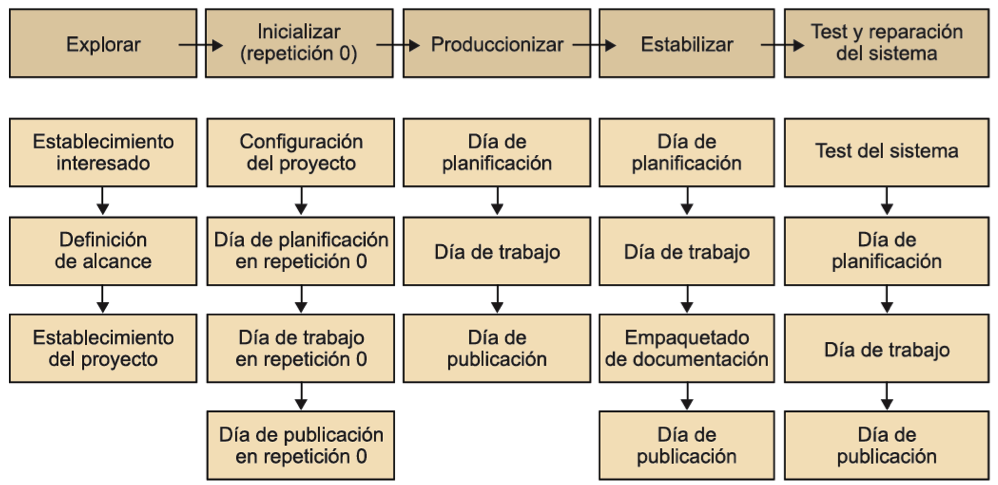
\includegraphics[width=1\textwidth]{Figuras/cicloDesarrollo.png}
		\rule{30em}{0.5pt}
	\caption[Ciclo de desarrollo de Mobile-D]{Ciclo de desarrollo de Mobile-D}
	\label{fig:cicloDesarrollo}
\end{figure}

\begin{itemize}
	\item \textbf{Exploración: }El propósito de la fase de exploración es planear y establecer el proyecto. Esta fase es importante para establecer las bases para la arquitectura del producto, la elección del entorno, y la implementación del sistema.
	\item \textbf{Inicialización: }El propósito de la fase de inicialización es posibilitar el éxito de las siguientes fases del proyecto preparando y verificando todos los problemas críticos del desarrollo, de manera que todos ellos sean corregidos con prontitud en el final de la fase de  aplicación de los requisitos. Además se preparan todos los recursos físicos, tecnológicos y de comunicaciones para las actividades de producción. 
	\item \textbf{Producción: }La fase de producción tiene como propósito implementar la funcionalidad requerida en el producto aplicando un ciclo de desarrollo iterativo e incremental. El desarrollo basado en pruebas es utilizado para implementar las funcionalidades.
	\item \textbf{Estabilización: }El propósito de la fase de estabilización es asegurar la calidad de la implementación del proyecto.
	\item \textbf{Pruebas del sistema: }El propósito de la fase de pruebas del sistema es comprobar si el producto implementa las funcionalidades requeridas correctamente, y corregir los errores encontrados.
\end{itemize}

Al analizar el método de desarrollo de software antes mencionado concluimos que es el adecuado para poder aplicarlo a nuestro sistema ya que necesitamos realizar iteraciones sobre un prototipo inicial y sobre ese trabajar para poder refinarlo hasta llegar al sistema final, es decir tendremos un avance paulatino en los requerimientos y desarrollo del mismo. \cite{MobileD} \cite{desDispositivos}